\documentclass[11pt, a4paper]{article}

\usepackage[left=2cm,text={17cm, 24cm},top=3cm]{geometry}
\usepackage[bottom]{footmisc}
\usepackage{times}
\usepackage[czech]{babel}
\PassOptionsToPackage{hyphens}{url}\usepackage[hidelinks]{hyperref}

\usepackage{graphicx}
\graphicspath{ {./} }

\begin{document}

\begin{titlepage}
    \begin{center}
        \textsc{\Huge Vysoké učení technické v Brně\\\vspace{0.5em}\huge Fakulta informačních technologií}
        
        \vspace{\stretch{0.382}}
        {\LARGE Modelování a simulace -- IMS\\\vspace{0.5em}}
        {\Huge T10: Počítačové služby}
        \vspace{\stretch{0.618}}
        
    \end{center}
    {\Large 2. 12. 2024 \hfill Lukáš Katona, Klára Kejdová}
\end{titlepage}

\newpage

\section{Úvod}

Cílém této studie je analyzovat sledování příspěvků na sociálních sítích a efektivita reklam na nich.
Různé skupiny lidí mají různé preference a zájmy, a proto se může stát,
že některé příspěvky nebudou dostatečně sledovány. Cílem je zjistit,
jakým způsobem se šíří informace a jakým způsobem se může zvýšit sledovanost reklam. 
Poznatky o šíření příspěvků mohou být využity pro zlepšení marketingových strategií.


Chtěli bychom sledovat, jak často sdílet a opakovat konkrétntí reklamu vzhledem rychlosti přibývajícíh, nových příspěvků na sociální síti
(poměr mezi reklamou a ostatními příspěvky), délkou příspěvků, časem zveřejnění a délkou doby pozornosti uživatelů.

\subsection{Co chceme sledovat:}
\begin{itemize}
    \item Kolik lidí dokouká příspěvek do konce
    \begin{itemize}
        \item Různé věkové kategorie idí mají jinou dobu pozornosti, proto délka příspěvku hraje roli v tom, jak je daný příspěvěk sledován.
        \item Optimalizací délky příspěšku můžeme zvýšit sledovanost.
    \end{itemize}
    \item Jaká je optimální délka příspěvu pro různé věkové skupiny
    \begin{itemize}
        \item V případě že uživatel nedokouká až do konce, pak nás zajímá, kolik procent příspěvku dokouká.
        \item Nejdůležitější informace by měly být na začátku příspěvku, aby je vidělo co nejvíce uživatelů.
    \end{itemize}
    \item Kolikrát uživatel vidí reklamu
    \begin{itemize}
        \item Pokud uživatel vidí danou reklamu málokrát, pak na ni nemusí reagovat.
        \item Přílišené opakování reklamy však může taktéž vést k negativní reakci.
    \end{itemize}
    \item Čas zveřejnění příspěvku 
    \begin{itemize}
        \item Čas zveřejnění v různé doby dne může mít vliv na sledovanost příspěvku.
        \item Pokud je příspěvek zveřejněn v době, kdy je uživatel online, pak je pravděpodobnější, že ho uvidí.
    \end{itemize}
\end{itemize}
% TODO k comu sme dospeli
% ako sme vysledky overovali

\newpage
\section{Fakta}

\subsection{Čas zveřejnění}
Dle \cite{TimeToPost}, jsme zjistili, že nejlepší čas na publikování příspěvků je zhruba mezi 9:00 - 12:00. Zde záleží na sociální síti, 
pro zjednodušení simulace budeme však používat průměrné hodnoty těchto časů.
Tento čas zároveň koreluje s naší vlastní zkušeností, kdy většina lidí bývá online.

\subsection{Délka příspěvku}
Délka příspěvku by měla záviset na schopnpsti lidí udržet pozornost. Záleží na co tito lidé upínají svoji pozornost,
naříklad, na práci se lidé soustředí déle než na sociální sítě, proto bylo náročené najít jednoznačné a konkrétní číslo.
Proto jsme hledali na více zdrojích a tato čísla zprůměrovali na základě našich vlastních zkušeností.

Podle \cite{AttentionSpan1}, starší lidé, přibližně nad 50 roků, mají průměrnou dobu pozornosti 2,5 minuty, zatímco lidé v produktivním věku mají pozornost již sníženou, a to na 40-75 sekund.
Na základě výzkumu \cite{AttentionSpan2}, mají děti pozornost ještě nižší, pouze 2-8 sekund.

\subsection{Opakování příspěvku a jejich sledovanost}
Tento bod je primárně důležitý z hleidska marketingu, aby se nestalo, že se reklamy stanou příliš otravnými.
Podle statustik \cite{SocialMediaAds}, pokud uživatel viděl danou reklamu 11krát a vícekrát, pak je o 10\% pravděpodobnější že na ni bude regovat negativně.
Navíc, pouze 44\% uživatelů dle \cite{SocialMediaAds-44} vidí nerelevantí reklamy. 

Je proto dlůežité, si dát pozor, jak často se budou příspěvky opakovat, aby nebyly otravné, ale zároveň aby byly dostatečně viděny.

\subsection{Hypotézy}
\begin{enumerate}
    \item Když uživatel tráví na sociální síti více času, je pravděpodobnější, že uvidí reklamu vícekrát a tedy by se měl snížit intervale opakování, aby nedošlo k negativní reakci.
    \item Pokud mají uživatelé nižší dobu pozornosti, pak by se měl snížit interval opakování, aby nedošlo k přílišnému shlédnutí reklamy.
    \item Pokud jsou příspěvky delší, pak jich uživatel uvidí za den méně, proto by se měl zvýšit interval opakování rekalmy.
    \item Interval opakování reklamy závisí na rychlosti přibývání nových příspěvků na sociální síti, čím rychleji přibývají, tím více by se měla reklama sdílet.
\end{enumerate}

\newpage
\section{Koncepce, způsob řešení}
Na ověření hypotéz jsme se rozhodli využít systém hromadné obsuhy, kde uživatel je linkou, která zpracovává příspěvky a reklamy (procesy).
Pro zakreslení konceptuiálního modelu jsme se rozhodli pro využití Petriho sítě. Simulační model jsme se rozdholdi na programovat v jazyce C++ s využitím knihovny SIMLIB\footnote{\href{https://www.fit.vut.cz/person/peringer/public/SIMLIB/}{https://www.fit.vut.cz/person/peringer/public/SIMLIB/}}.
\subsection{Konceptuální model}
Uživatel je obslužnou linkou, která zpracovává příchozí příspěvky a reklamy. Ty přicházejí do systému, kde se dostávají na zásobník,
to znamená že novější příspěvky mají priotiu a může se stát že k některým příspěvkům uživatel ani nedojde.
Pokud příspěvěk trvá déle, jako je doba pozornosti uživatele, pak jej uživatel nedokouká do konce a příspěvek opouští systém.
Pokud jej ale dokouká dokonce, tak stále záleží na jeho relevanci, zda uživatele zaujal a na něj uživatel reaguje, v ten moment příspěvek opouští systém jako relevantní nebo ne.
Dále je také v případě reklamy sledováno, kolkrát ji uživatel za den viděl.
Pokud to bylo příliškrát, pak se o tom vytváří záznam.

Uživatel má také svou dobu, kdy je online, nejaktivnější je mezi 9:00 - 12:00, jinak je méně aktivní, nebo není aktivní vůbec, například když spí.
Jeho aktiviu ovlivňuje běžné denní aktivity, jako je práce, škola, nebo volný čas. Když je člověk aktivnější, pak na sociální síti tráví delší dobu a přestávky jsou kratší.
Pokud je uživatel méně aktivní je jeho doba na sociální stíti kratší a přestávky jsou delší. Pokud uživatel spí, pak je offline a neodebírá žádně příspěvky.

Pro zjednodušení zanedbáváme různé dny v týdnu, kdy se může chování uživatele lišit. Taktéž, když se naplní počítalo reklam za den, tak jej resetujeme,
což znamená že uživatel může vidět reklamu znovu další den.
%V našem modelu existuje pouze jeden zásobník pro příspěvky, který je sdílený.
Máme sdílený zásobík pro příspěvky a reklamy, tyto jednotlivé procesy si v sobě nesou informaci o svém typu, který ovlivňuje chování systému.

\subsubsection{Proměnné paramtery modelu}
Náš model obsahuje různé proměnilvé paramtery, které se budou pro jednotlivé experimenty měnit pro ověření hypotéz.
Na základě nastavené interval generování nových příspěvků, doby příspěvku a doby pozornosti se budeme snažit najít optimální interval pro generování reklam.
\begin{itemize}
    \item Interval mezi generováním nových příspěvků
    \item Interval mezi generováním reklam
    \item Doba příspěvku
    \item Doba pozornosti
\end{itemize}

\subsubsection{Petriho síť}
\vspace{1em}
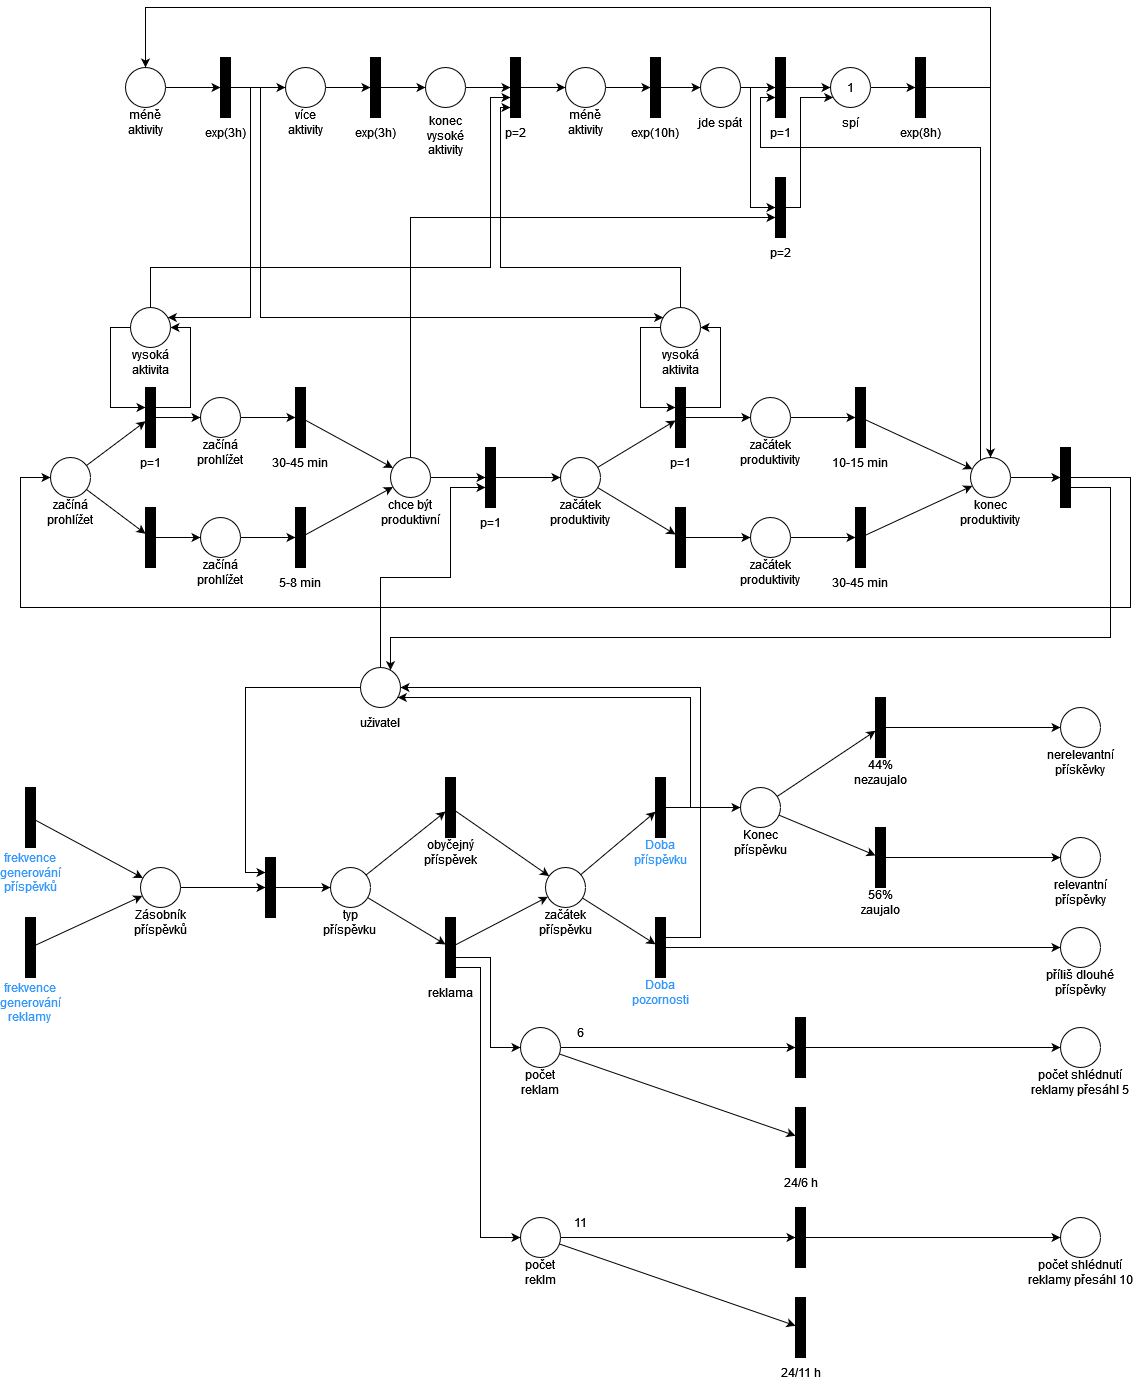
\includegraphics[width=\linewidth]{petri-net.png}
\vspace{1em}

\subsection{Simulační model}
Simulační model jsme imlementovali v jazyce C++ s využitím knihovny SIMLIB\footnote{\href{https://www.fit.vut.cz/person/peringer/public/SIMLIB/}{https://www.fit.vut.cz/person/peringer/public/SIMLIB/}}.
\subsubsection{Proces: DayPhaseManager}
Proces, který řídí denní fáze uživatele, kdy je na sociálnísítí více aktivní, kdy méně a kdy vůbec. 
Má 24 hodinový cyklus, během kterého se vystřídá několik fází, ráno, dopoledne, odpoledne, a noc, během které uživatel spí.
Spánek je vždy dopočítám dle doby denních aktivit tak, aby uživatel vstával vždy v 6:00 a tím započal nový den.
\subsubsection{Proces: UserActivityManager}
Tento proces mění aktivity uživatele mezi produktivitou a časem ztráveným na sociálních sítích, přičemž doby trvání daných činností se mění na základě denní fáze.
\subsubsection{Proces: Post (Příspěvek)}
Post je proces, který reprezentuje jednotlivé příspěvky na sociální síti. Má svou dobu trvání, která se generuje v rozmezí obyvklé doby příspevků.
Zároveň řeší dobu pozornosti uživatele, pokud je kratší než doba trvání příspěvku, pak uživatel příspěvek nedokouká do konce.
Na základě přeskočení příspěvku nebo jeho dokoukání, se zaznamenává jeho relevantnost.
\subsubsection{Proces: PostGenerator}
Generuje nové příspěvky na sociální síti v závislosti na nastaveném intervalu, včetně jeho náhodné délky.
\subsubsection{Proces: Ad (Reklama)}
Reprezentuje proces reklamy, která se zobrazí uživateli. Funguje podobně jako Post, tedy řeší délku, pozornost uřivatele, ale zahrnuje navíc únavu z většího počtu reklam a případnou autoregulaci.
\subsubsection{Proces: AdGenerator}
Funguje téměř stejně jako PostGenerator, ale generuje reklamy na základě upravéného času pomcí autoregulace. Pokud uživatel viděl reklamu příliškrát, pak se zvýší interval jejího generování, aby ji uživatel viděl méněkrát.
\subsubsection{Událost: AdArrivalTimeRegulation}
Událost, která reguluje interval zobrazení reklam na základě počtu reklam, kdy každý den sníží počet reklam o jedna.
\subsubsection{Událost: AdFatigueDecrementor}
Událost, která snižuje počet již shlédnutých reklam každých 24/6 hodin, aby se mohly zobrazit znovu další den. Počítáme totiž 6 reklam ne za den, ale za 24 hodin od první reklamy.


\section{Testování, experimenty}

\section{Závěr}

\bibliographystyle{czechiso}
\bibliography{reference}
    
\end{document}